\begin{figure*}[b]
\centering
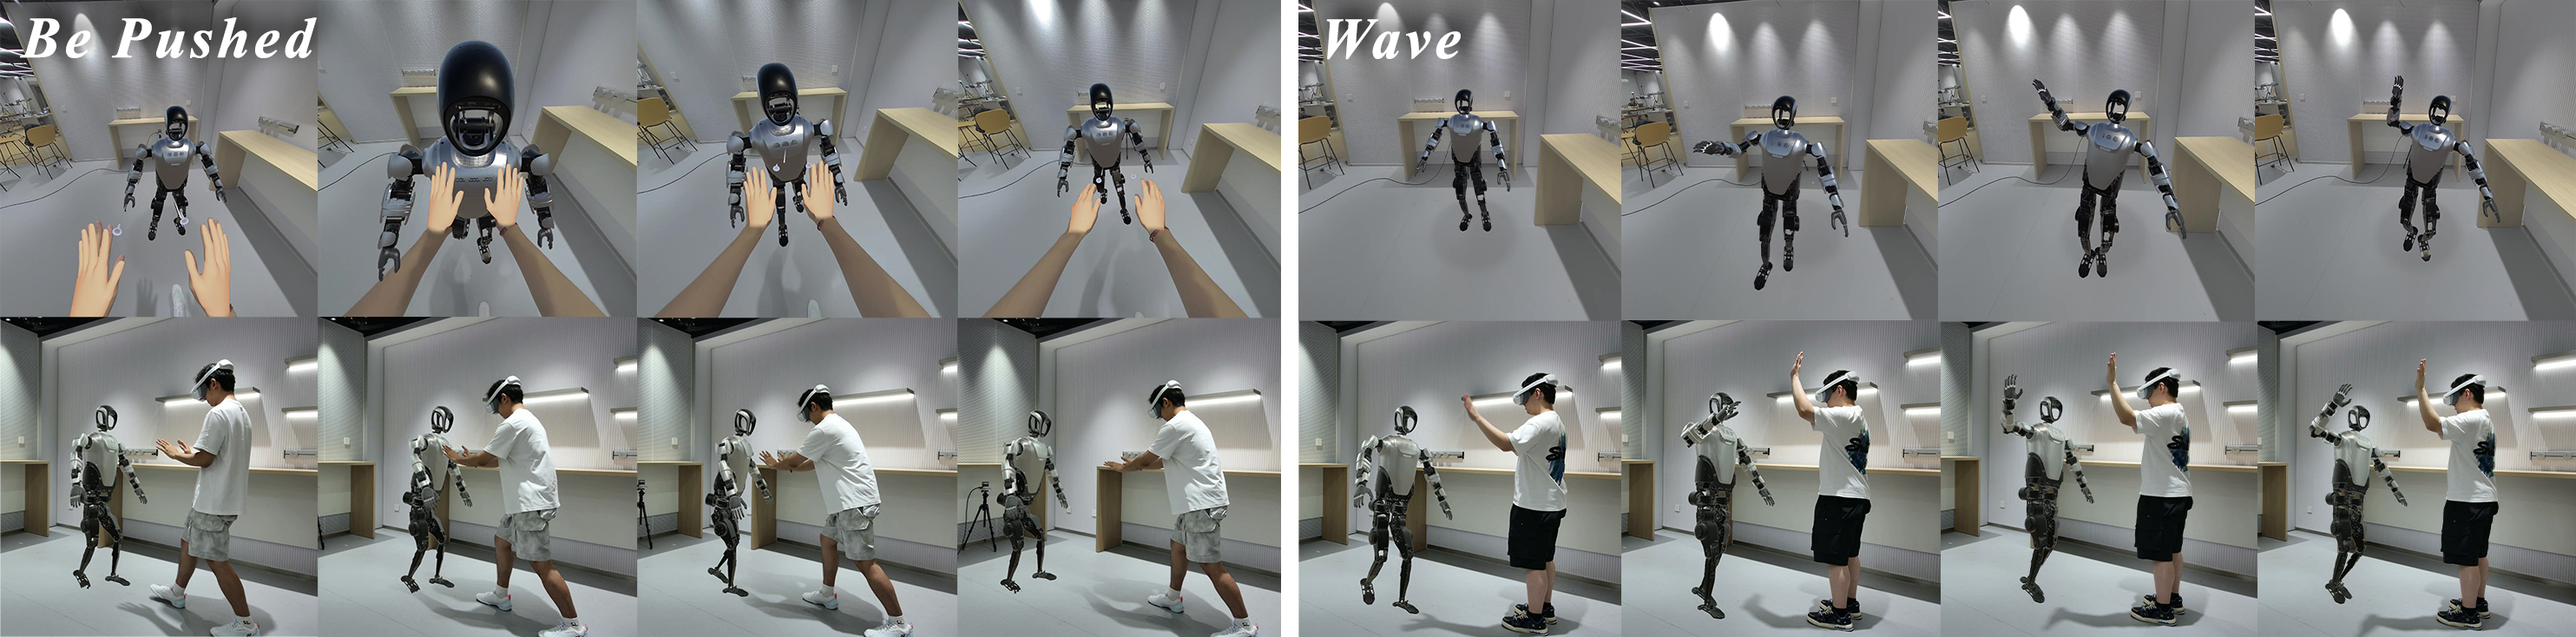
\includegraphics[width=1.0\linewidth]{images/interact.png}
\vspace{-20px}
\caption{The human-robot interactions presented in our system. Top: The first-person perspective visualized via the AR glasses. Bottom: The third-person perspective produced by fusing the captured human user in the physical environment and the rendered virtual robot.}
\label{fig:systeminter}
\end{figure*}

\begin{figure*}[h]
\centering
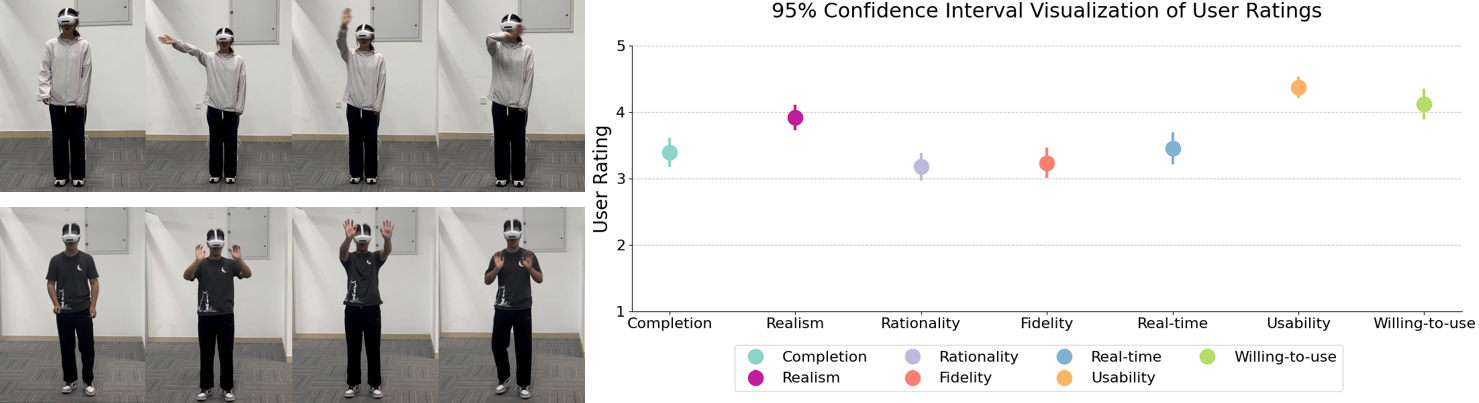
\includegraphics[width=1.0\linewidth]{images/reeeeeee.png}
\vspace{-20px}
\caption{Process and results of the user empirical test. Left: Participants interacting with virtual robots via our system. Right: The 95$\%$ confidence interval visualization of user ratings showing the mean and boundary of the confidence intervals. Here, 1 indicates "poor" and 5 indicates "excellent".}
\label{fig:userstudy}
\end{figure*}
\vspace{-20px}
\begin{figure*}[b]
\centering
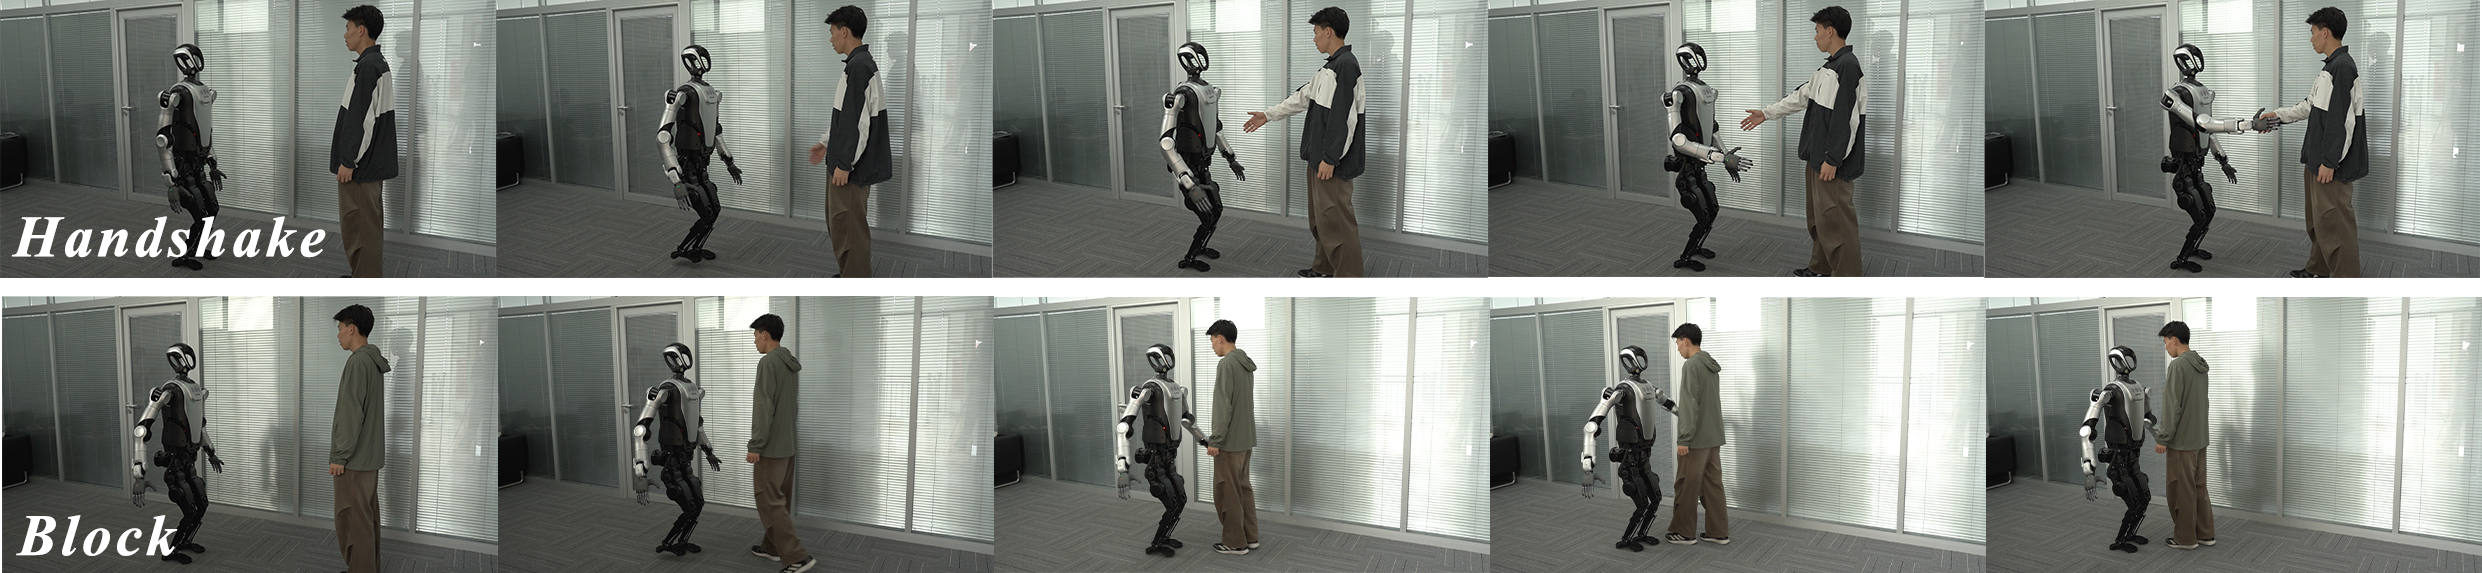
\includegraphics[width=1.0\linewidth]{images/physicalrobot.png}
\vspace{-20px}
\caption{A real LEJU Kuavo robot performing the robot movements generated by the robotic interaction model. Since the real robot exhibits a high consistency with the appearance of the virtual robot shown in our system, a human user can easily and smoothly interact with the real robot.}
\vspace{-20px}
\label{fig:realrobot}
\end{figure*}